\chapter{SOMHunter Architecture}
\label{arch}


When we say SOMHunter, we usually mean the main part of the project --- as visualized in the~\cref{fig:sh-arch}, with the label "SOMHuner Video Search Tool". Of course, it is nothing without the data to work on. The extracted dataset is generated by the extraction pipeline before actually launching the tool.

Currently, SOMHunter has four separated parts --- \emph{Core}, \emph{GUI}, \emph{data server} and \emph{ranking server}.


\begin{figure}[b]
	\centering
	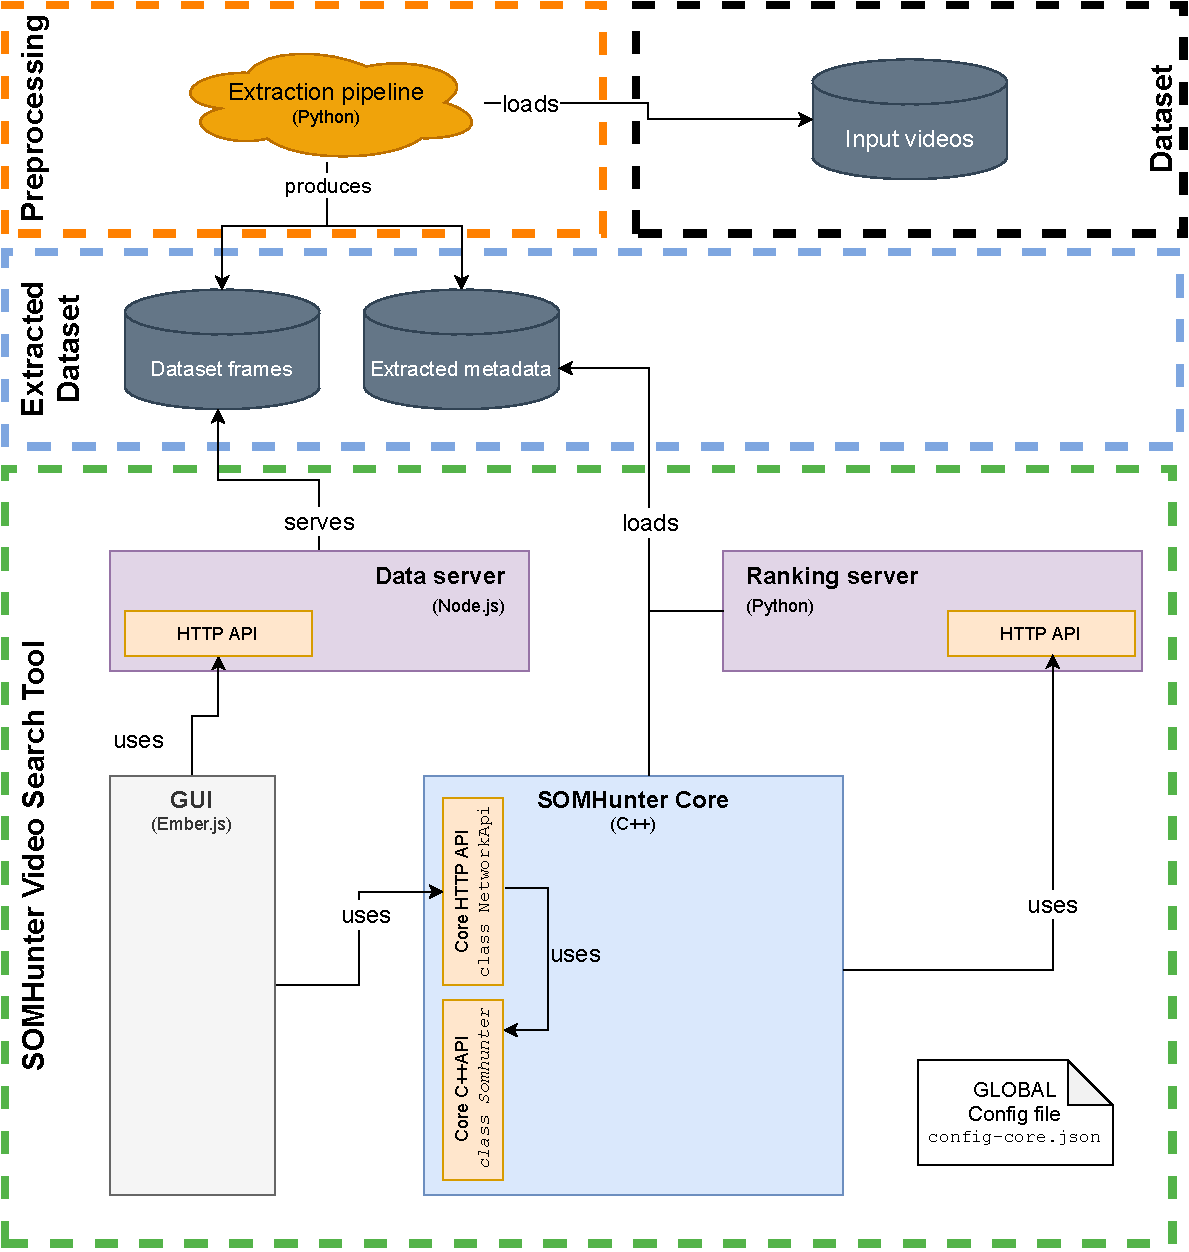
\includegraphics[width=1.0\textwidth]{img/diagrams/sh-arch.pdf}
	\caption{\textbf{High-level architecture of the SOMHunter tool.} Showing also extraction pipeline and visualising the path of the input dataset.}
	\label{fig:sh-arch}
\end{figure}

\section{Core}

The core is a stand-alone C++ piece of software that does all the hard work related to the search. In short, every search is represented and managed inside the core. The core is the director of everything here and the remaining components are just stateless services or helpers.

It loads the extracted dataset and holds the state of the ongoing search. It does all the query scoring, generates displays, handles all the logging and optionally communicates with a remote evaluation server (usually during the competitions). Every time a user does something, the core is notified either through C++ or HTTP API and it changes its state accordingly. 

More details about the core can be found in~\cref{comp-core}.

\section{UI}

More on that in~\cref{comp-ui}.

\section{Data Server}

More on that in~\cref{comp-data-server}.

\section{Ranking Server}

More on that in~\cref{comp-ranking-server}.


\section{Other Component}
As we mentioned earlier, beside the tool itself there are other parts that are essential for the tool.

\subsection{Extraction Pipeline}

More on that in~\cref{extraction-pipeline}.

\subsection{Extracted Dataset}

More on that in~\cref{extracted-dataset}.


\subsection{SOMHunter Simulator}

\subsection{Log Analyzer}


